\documentclass[10pt,a4paper]{article}
\usepackage{graphicx,geometry}
\usepackage{listings}
\usepackage{color}
\usepackage[many]{tcolorbox}
\usepackage{amsmath}
\usepackage{longtable}
\usepackage{lscape}
\usepackage{subcaption}
\definecolor{dkgreen}{rgb}{0,0.6,0}
\definecolor{gray}{rgb}{0.5,0.5,0.5}
\definecolor{mauve}{rgb}{0.58,0,0.82}
\begin{document}

\title{COL 718 - LAB2 \\ \textbf{Simulating a system with 2 caches(L1 and L2) for Different Parameters} \\ Submitted to: Prof. Kolin Paul \\ IIT Delhi}

\author{Madhur Aswani \cr 2023JVL2241}

\date{\today}

\maketitle
\section{Introduction}
In this LAB I simulated a system with CPU Type \emph{Timing} and different Cache parameters operating at a fixed frequency of \emph{600MHz}. The aim of this lab is to see how different parameters of the cache affect the system.
\section{Experimental Details}
In this Experiment, I have added two L1 Caches and one L2 Cache. The 2 L1 Caches are \textbf{L1ICache} and \textbf{L1DCache} each specifically connected to CPU \emph{ICache} port and \emph{DCache} port respectively. The CPU sends the Instruction requests to \textbf{L1ICache} and data requests \textbf{L1DCache}. For this experiment, the size of \textbf{L1ICache} has been fixed at \emph{16kB}. In comparison, the other cache parameters are varied equally over both the L1Catches.
\subsection{Parameters of Experiment}
We are going to vary the below parameters in this experiment -
\begin{itemize} 
\item \textbf{L1nL2ratio} - It refers to the ratio of sizes of L1 and L2 cache in the system [2, 4, 8, 16].
\item \textbf{L1Latency} - It is the Latency of L1 Cache in num of cycles [1-5].
\item \textbf{L2Latency} - It is the Latency of L2 Cache in num of cycles [10, 15, 20, 25, 30].
\item \textbf{L1assoc} - It is the associativity of L1 Cache [2, 4, 8].
\item \textbf{L2assoc} - It is the associativity of L2 Cache [4, 8, 16].
\item \textbf{L1Size} - It is the Size of L1 Cache ['64kB', '128kB'].
\item \textbf{blkSize} - When given 0 it uses unblocked MM and is varied for 4 and 8 block sized MM.
\end{itemize}
\subsection{Stats Focused}
In this experiment, I will be focusing on the below statistics - 
\begin{itemize} 
\item \textbf{simSeconds} - This stat gives the simulated seconds of the system.
\item \textbf{hostInstRate} - This state gives the simulator instruction rate (inst/s) ((Count/Second))
\item \textbf{numCycles} - Number of CPU cycles simulated (Cycle)
\item \textbf{cpu.cpi} - CPI: cycles per instruction (core level) ((Cycle/Count))
\item \textbf{cpu.ipc} - IPC: instructions per cycle (core level) ((Count/Cycle))
\item \textbf{dcache.overallMissRate::total} - The stat gives the Overall Miss Rate of \emph{L1DCache}.
\item \textbf{dcache.overallAvgMissLatency::total} - The stat gives the Overall Avg Miss Latency of \emph{L1DCache}.
\item \textbf{icache.overallMissRate::total} - The stat gives the Overall Miss Rate of \emph{L1ICache}.
\item \textbf{icache.overallAvgMissLatency::total} - The stat gives the Overall Avg Miss Latency of \emph{L1Cache}.
\item \textbf{l2cache.overallMissRate::total} - The stat gives the Overall Miss Rate of \emph{L2Cache}.
\item \textbf{l2cache.overallAvgMissLatency::total} - The stat gives the Overall Avg Miss Latency of \emph{L2Cache}.
\end{itemize}
\subsection{Methodology}
In this experiment, I have created a system with a \emph{X86TimingSimpleCPU} CPU and 2 L1 Catches, one for Instruction and one for Data. Apart from this, there is an L2 Cache. Everything is specified in the \emph{Config.py} file in Appendix \ref{appendix:Code Files}. There is also a \emph{Cache.py} which defines the cache settings. For workload, I am using MM of $25 \times 25$ Matrix and have added blocksize as an argument to the binary generated. The code is given in Appendix \ref{appendix:Code Files}. I have also written a \emph{bash.sh} file to automate the simulation for different parameters and store the generated stat files.

\section{Results}
After running the bash file, I obtained about 288 stat files and created a script that writes the stats listed in these stat files to a combined \emph{Data.csv} file. I have obtained some interesting plots from the file and observed the below.
\begin{itemize}
\item As the \emph{blkSize} Increases the \emph{dcache.overallMissRate::total} decreases with the unblocked MM having the highest missing rate. There is a significant decrease when we start using blocked MM.

\begin{figure}[h!]
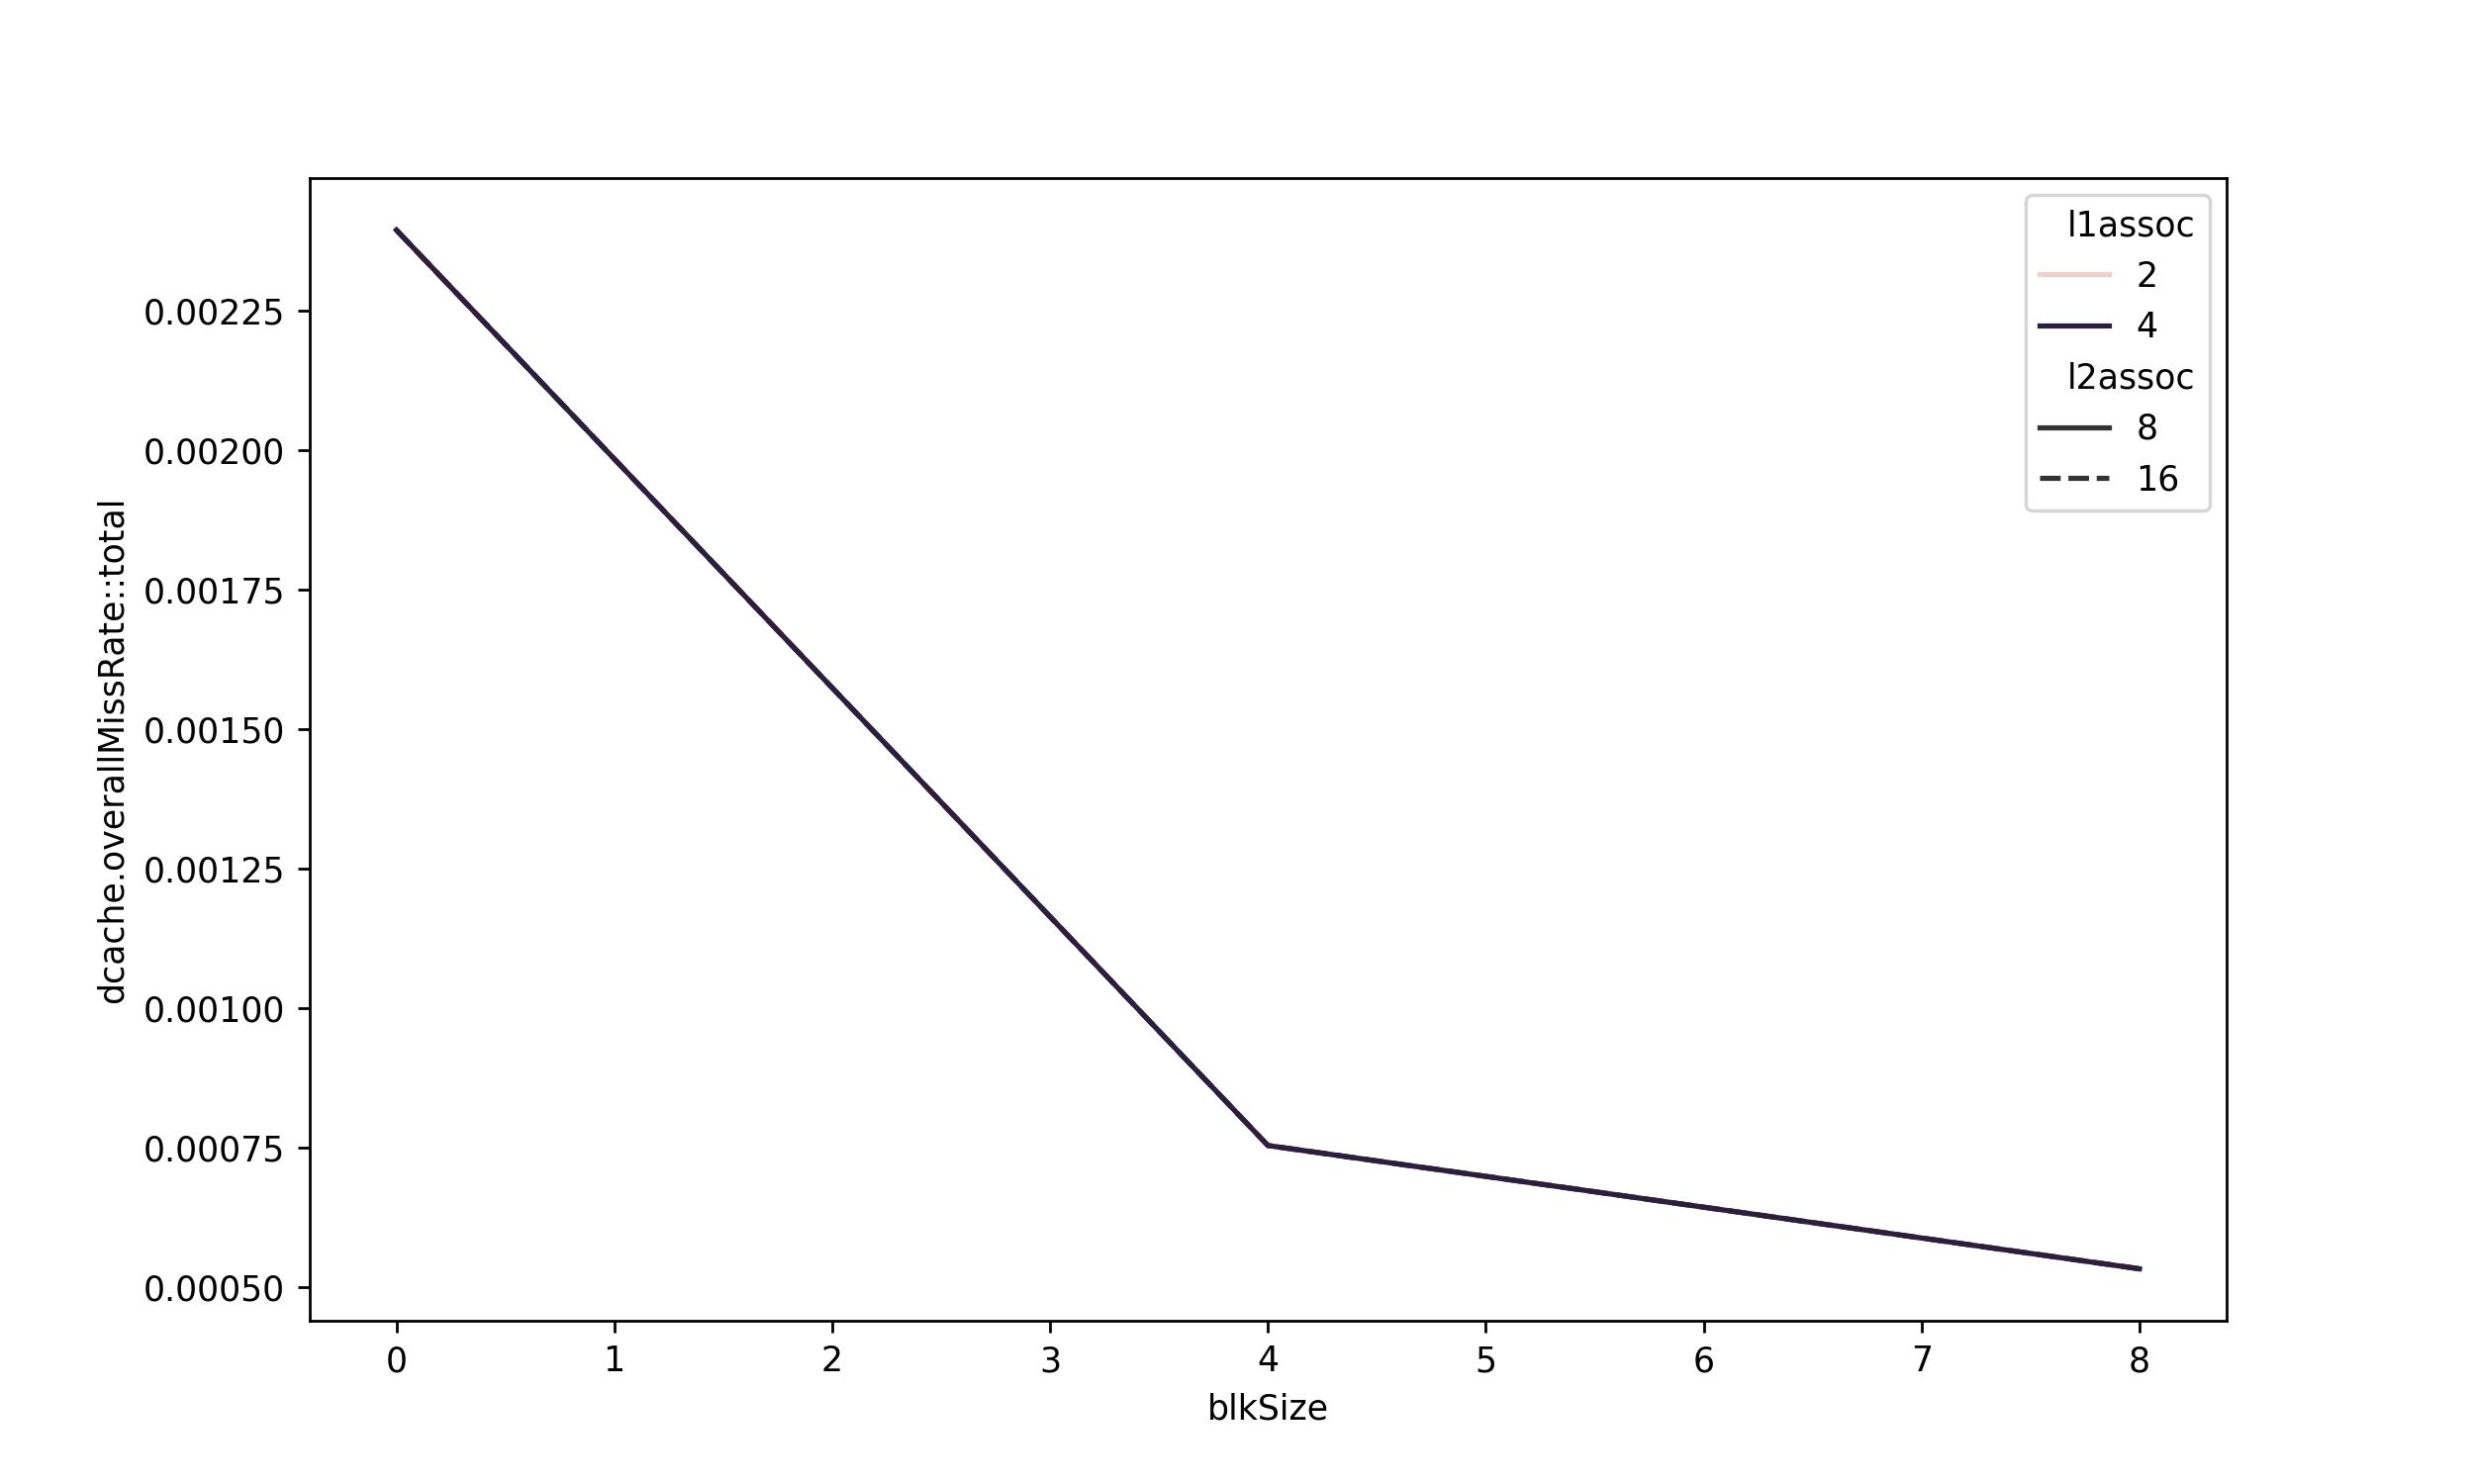
\includegraphics[width=\linewidth]{figures/blkSize-VS-dcacheMissRate_64KB_lineplot.jpg}
\caption{A Lineplot of blkSize and dcacheMissRate}
\end{figure}
\item The plot of \emph{hostInstRate} with \emph{blockSize} for different associativity of l1, l2 and size of l1 cache show changed behavior. For an \emph{l1assoc} of 2, \emph{l2assoc} of 8 and \emph{l1Size } of 64kB, the unblocked MM performs the best with the highest  \emph{hostInstRate}. As we start using Blocked MM, it still remains the highest for a block size of 4 but on using eight block size the configuration of \emph{l1assoc} of 4 and \emph{l2assoc} of 16 has the highest \emph{hostInstRate}. Whereas for 128KB of cache size the \emph{l1assoc} of 4 and \emph{l2assoc} of 16 had the highest \emph{hostInstRate}, but if we move to block size of 8, we observe that the configuration of \emph{l1assoc} of 4 and \emph{l2assoc} of 8 has the highest \emph{hostInstRate}.
\begin{figure}[h!]
\begin{subfigure}{.5\textwidth}
\includegraphics[width=\linewidth]{figures/blkSize-VS-hostInstRate_64KB_lineplot.jpg}
\caption{A Lineplot of blkSize and hostInstRate for 64kB}
\end{subfigure}
\begin{subfigure}{.5\textwidth}
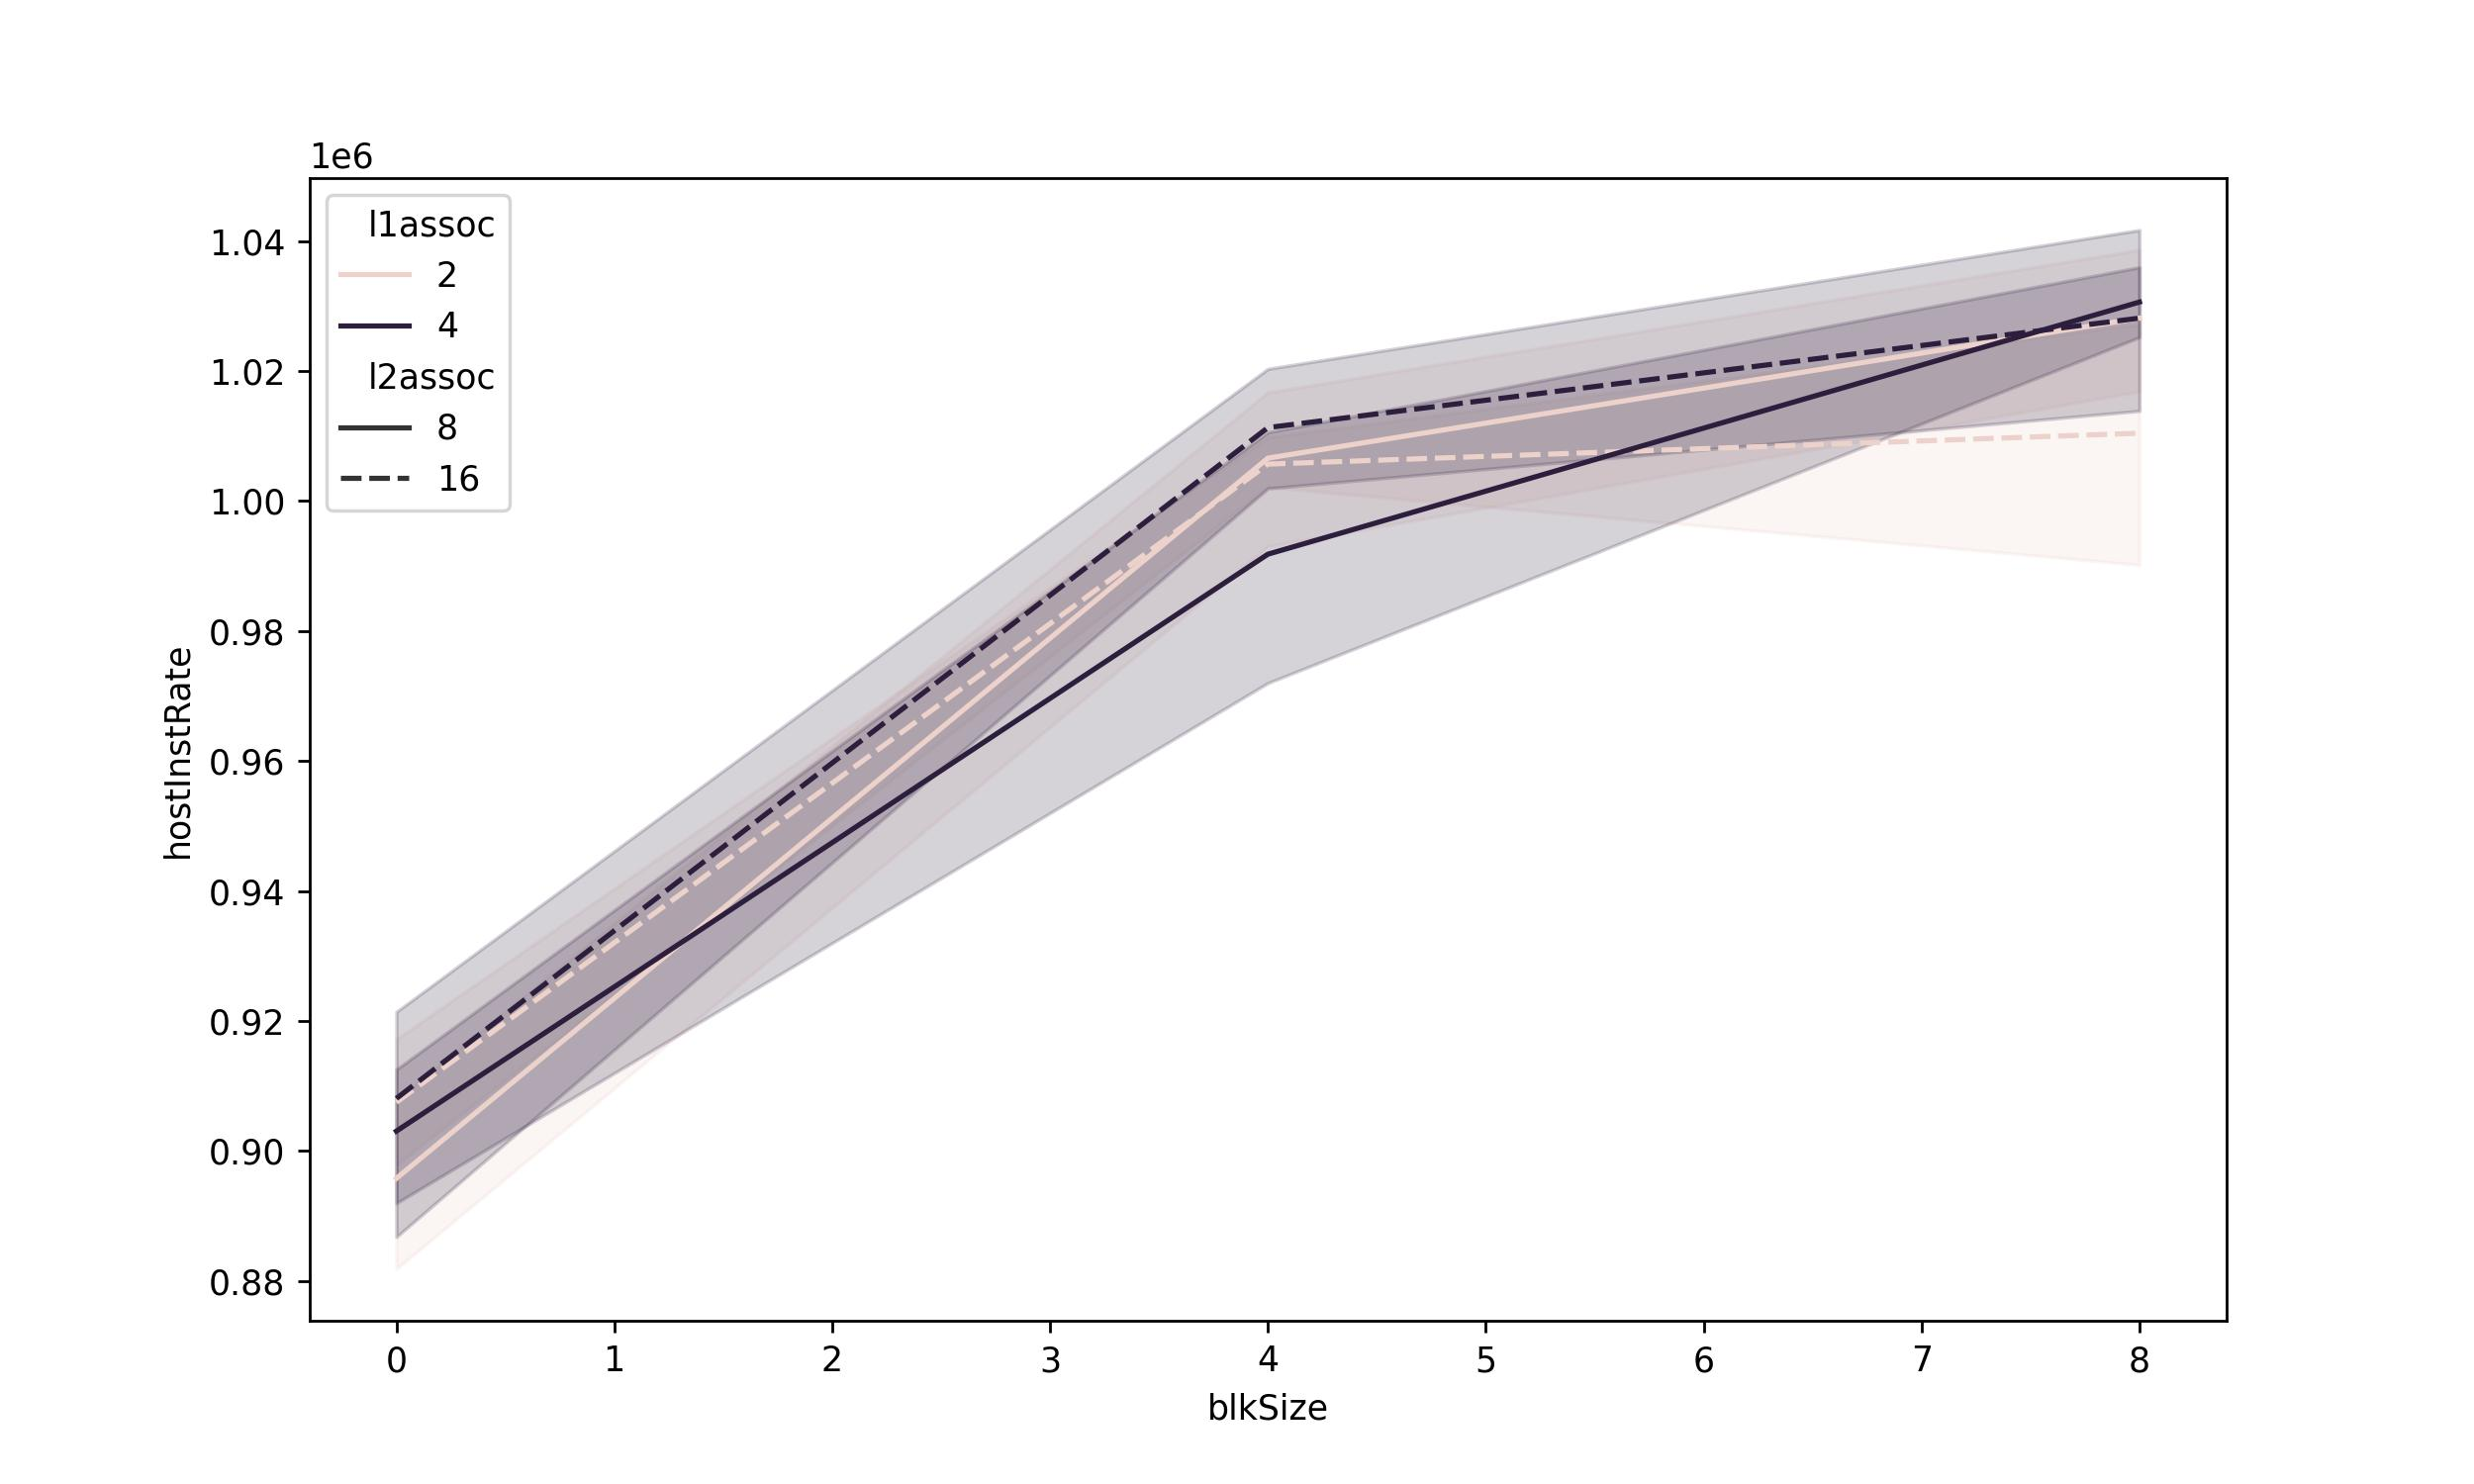
\includegraphics[width=\linewidth]{figures/blkSize-VS-hostInstRate_128KB_lineplot.jpg}
\caption{A Lineplot of blkSize and hostInstRate for 128kB}
\end{subfigure}
\end{figure}
\item From the above, it seems that the \emph{simSeconds} should decrease as the block size increases, but if you plot them, the entire opposite is observed. I guess the number of operations is high in case of blocked due to 6 nested for loops in the code.
\begin{figure}[h!]
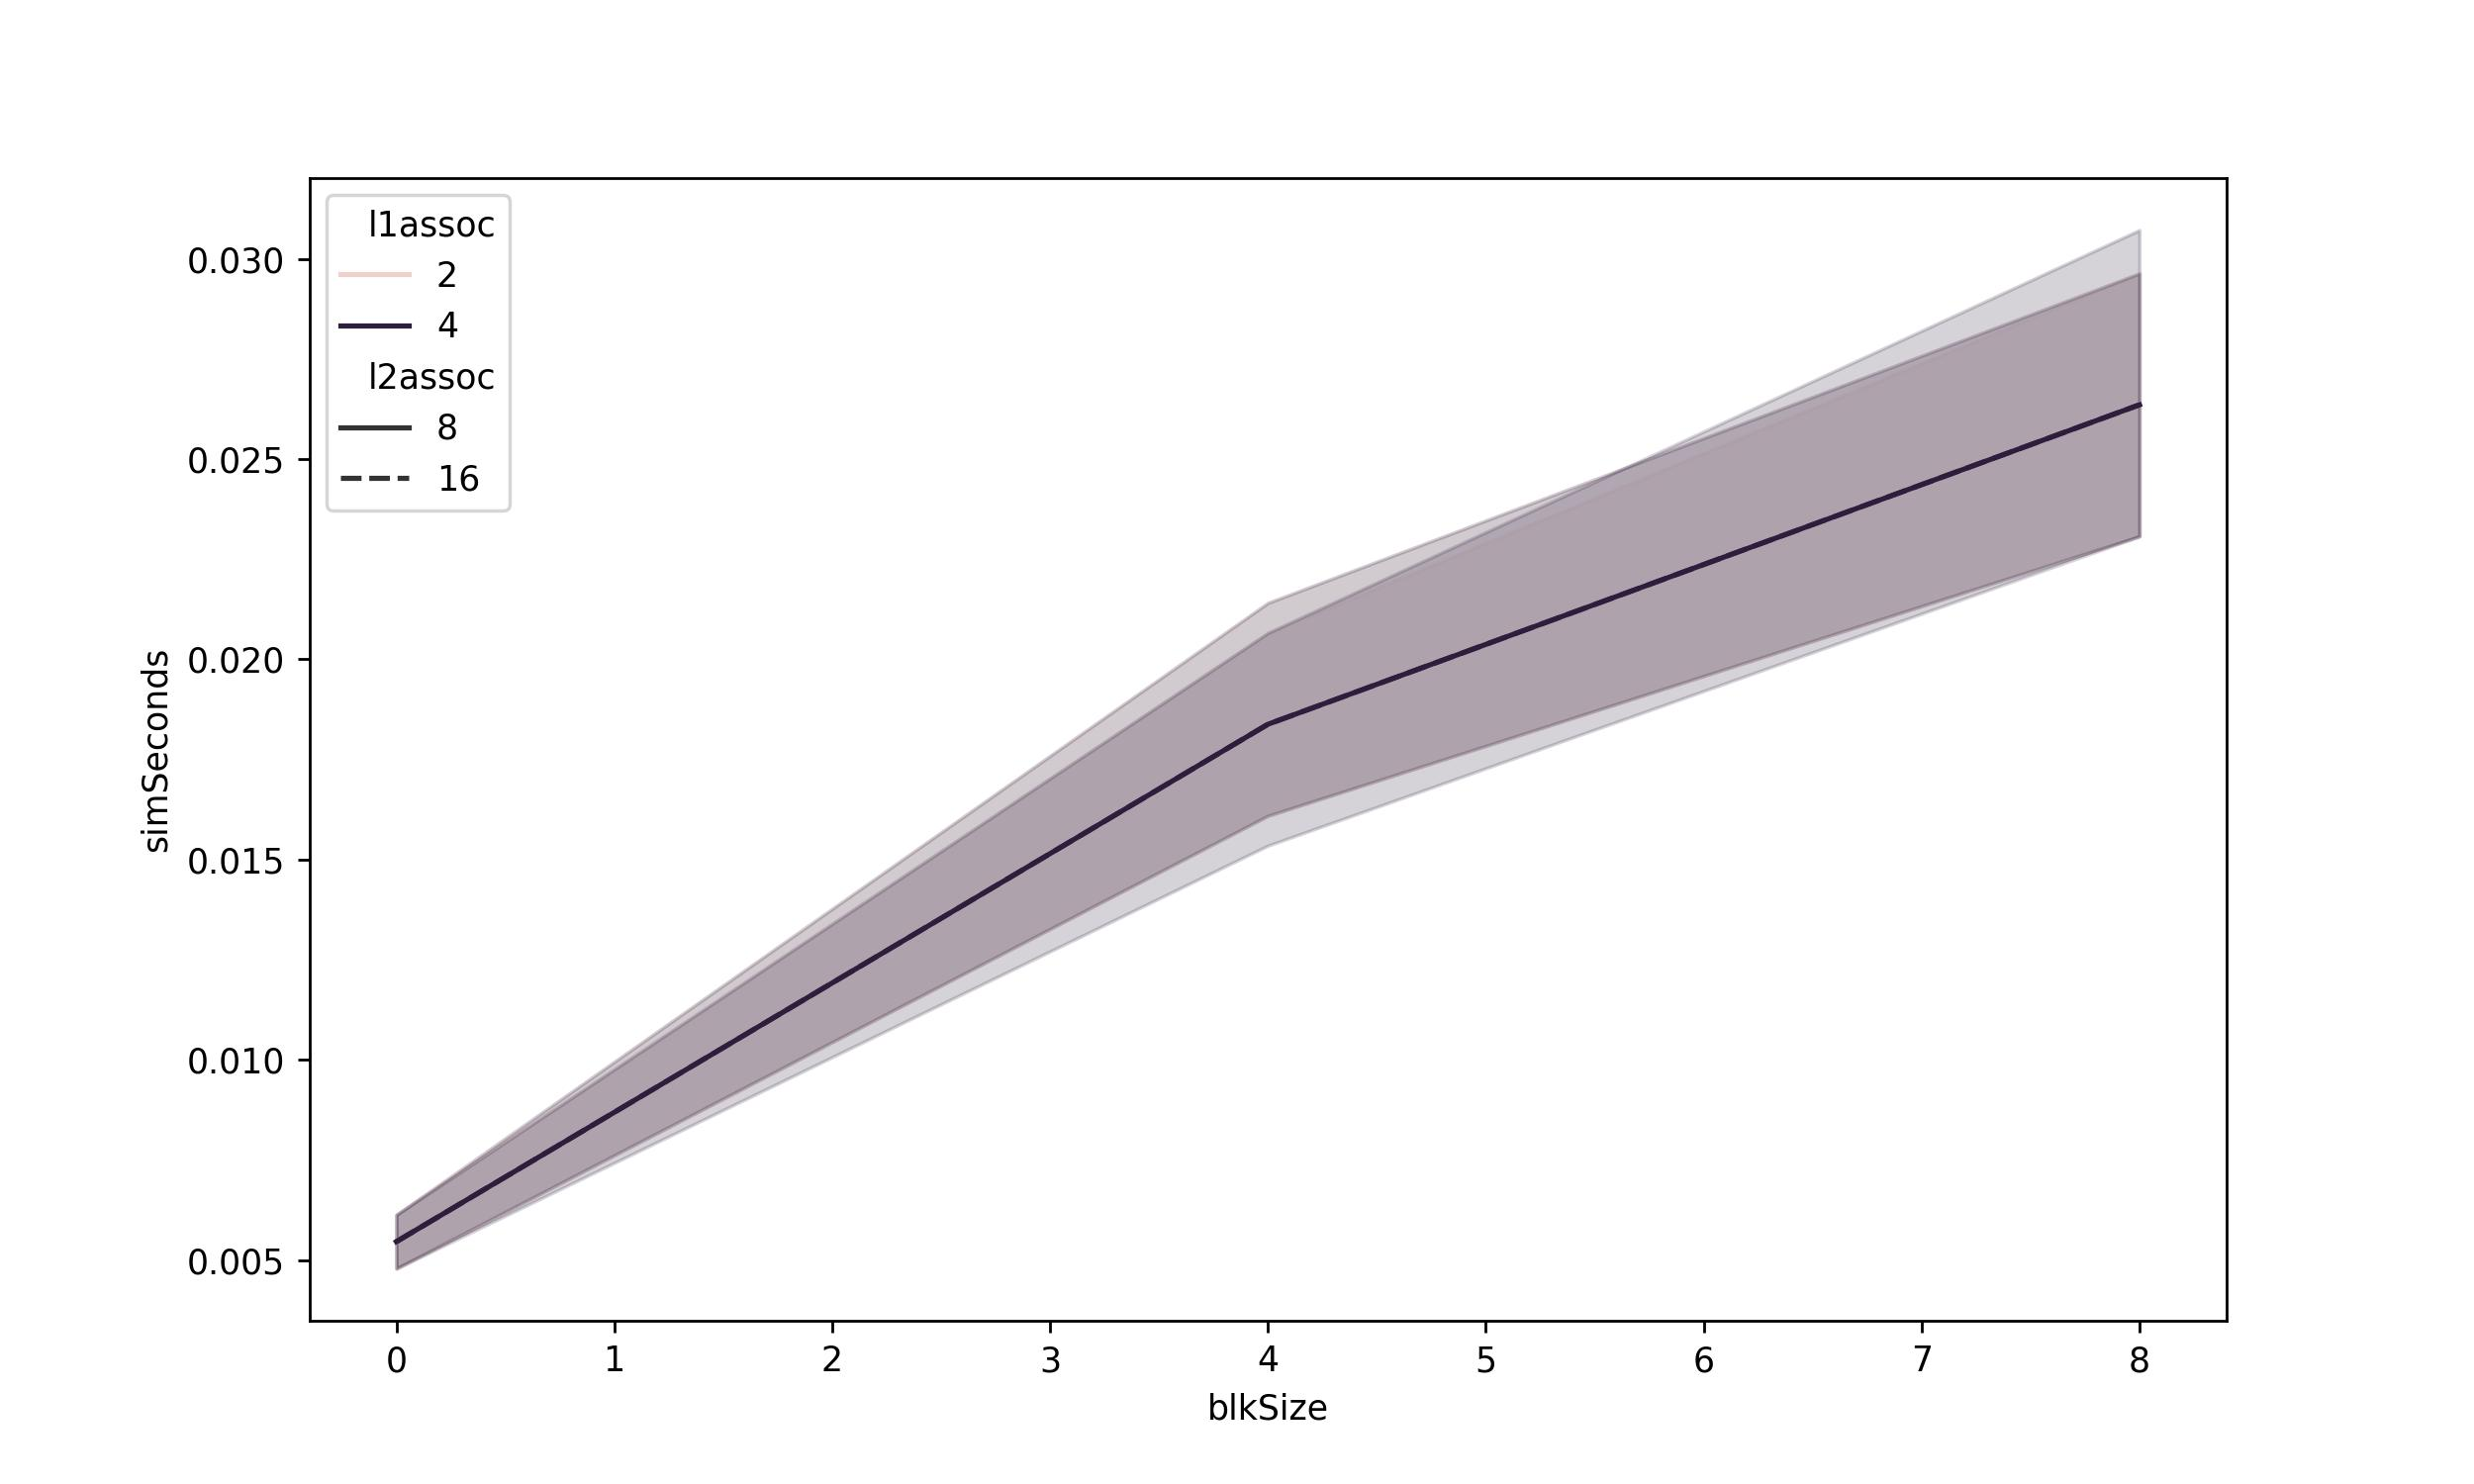
\includegraphics[width=\linewidth]{figures/blkSize-VS-simSeconds_64KB_lineplot.jpg}
\caption{A Lineplot of blkSize and simSeconds}
\end{figure}
\end{itemize}
\clearpage
\appendix

\section{Code Files}\label{appendix:Code Files}
\textbf{Config.py}
\lstset{frame=tb,
   language=Python,
   aboveskip=3mm,
   belowskip=3mm,
   showstringspaces=false,
   columns=flexible,
   basicstyle={\small\ttfamily},
   numbers=none,
   numberstyle=\tiny\color{gray},
   keywordstyle=\color{blue},
   commentstyle=\color{dkgreen},
   stringstyle=\color{mauve},
   breaklines=true,
   breakatwhitespace=true
   tabsize=3
   }
\begin{lstlisting}
import m5
from m5.objects import *
import argparse
from Cache import *

parser = argparse.ArgumentParser(description='Config For Simulation')
parser.add_argument("-f","--freq",type=str)
parser.add_argument("--l1Size",type=str)
parser.add_argument("--l2Ratio",type=float)
parser.add_argument("--l1assoc",type=int)
parser.add_argument("--l2assoc",type=int)
parser.add_argument("--blksize",type=str)
parser.add_argument("--l1Latency",type=int)
parser.add_argument("--l2Latency",type=int)






args=parser.parse_args()
size_l1=args.l1Size
l1s=int(size_l1[:-2])
l2s=l1s*args.l2Ratio
l2Size=str(int(l2s))+"kB"
system = System()
l1Icache=L1Cache(args.l1assoc,args.l1Latency,size='16kB')
l1Dcache=L1Cache(args.l1assoc,args.l1Latency,size=args.l1Size)
l2Cache=L2Cache(assoc=args.l2assoc,latency=args.l2Latency,size=l2Size)


system.clk_domain = SrcClockDomain()
system.clk_domain.clock = args.freq
system.clk_domain.voltage_domain = VoltageDomain()

system.mem_mode = 'timing'
system.mem_ranges = [AddrRange('1GB')]

system.cpu = X86TimingSimpleCPU()

system.cpu.icache = l1Icache
system.cpu.dcache = l1Dcache

system.cpu.icache.cpu_side=system.cpu.icache_port
system.cpu.dcache.cpu_side=system.cpu.dcache_port

system.l2bus = L2XBar()

system.cpu.icache.connectBus(system.l2bus)
system.cpu.dcache.connectBus(system.l2bus)

system.l2cache = l2Cache
system.l2cache.connectCPUSideBus(system.l2bus)
system.membus = SystemXBar()
system.l2cache.connectMemSideBus(system.membus)

system.cpu.createInterruptController()
system.cpu.interrupts[0].pio = system.membus.mem_side_ports
system.cpu.interrupts[0].int_requestor = system.membus.cpu_side_ports
system.cpu.interrupts[0].int_responder = system.membus.mem_side_ports

system.system_port = system.membus.cpu_side_ports

system.mem_ctrl = MemCtrl()
system.mem_ctrl.dram = DDR3_1600_8x8()
system.mem_ctrl.dram.range = system.mem_ranges[0]
system.mem_ctrl.port = system.membus.mem_side_ports

system.workload = SEWorkload.init_compatible("../../Github/IITD_Learning/Architecture of HPC/LAB2/loadBinary")

process = Process()
process.cmd=["../../Github/IITD_Learning/Architecture of HPC/LAB2/loadBinary",args.blksize]
system.cpu.workload = process
system.cpu.createThreads()
root = Root(full_system = False, system = system)
m5.instantiate()

print("Beginning simulation!")
exit_event = m5.simulate()

print('Exiting @ tick {} because {}'.format(m5.curTick(), exit_event.getCause()))



\end{lstlisting}
\textbf{Cache.py}
\begin{lstlisting}
from m5.objects import Cache

class L1Cache(Cache):
    assoc = 2
    data_latency = 2
    tag_latency = 2
    response_latency = 2
    mshrs = 4
    tgts_per_mshr = 20
    size='64kB'
    def __init__(self,assoc,latency,size):
        super(L1Cache, self).__init__()
        self.assoc=assoc
        self.data_latency=latency
        self.tag_latency=latency
        self.response_latency=latency
        self.size=size
    def connectBus(self, bus):
        self.mem_side = bus.cpu_side_ports


class L2Cache(Cache):
    assoc = 8
    tag_latency = 20
    data_latency = 20
    response_latency = 20
    mshrs = 20
    tgts_per_mshr = 12
    
    size='256kB'
    def __init__(self,assoc,latency,size):
        super(L2Cache, self).__init__()
        self.assoc=assoc
        self.data_latency=latency
        self.tag_latency=latency
        self.response_latency=latency
        self.size=size
    def connectCPUSideBus(self, bus):
        self.cpu_side = bus.mem_side_ports

    def connectMemSideBus(self, bus):
        self.mem_side = bus.cpu_side_ports
\end{lstlisting}
\textbf{load.c}
\lstset{frame=tb,
   language=Python,
   aboveskip=3mm,
   belowskip=3mm,
   showstringspaces=false,
   columns=flexible,
   basicstyle={\small\ttfamily},
   numbers=none,
   numberstyle=\tiny\color{gray},
   keywordstyle=\color{blue},
   commentstyle=\color{dkgreen},
   stringstyle=\color{mauve},
   breaklines=true,
   breakatwhitespace=true
   tabsize=3
   }
\begin{lstlisting}
#include <stdio.h>

int main(int argc, char* argv[]){


int res[25][25];
int sum;
int block=atoi(argv[1]);


int a[25][25]={{1, 2, 3, 4, 5, 6, 7, 8, 9, 10, 11, 12, 13, 14, 15, 16, 17, 18, 19, 20, 21, 22, 23, 24, 25}, {1, 2, 3, 4, 5, 6, 7, 8, 9, 10, 11, 12, 13, 14, 15, 16, 17, 18, 19, 20, 21, 22, 23, 24, 25}, {1, 2, 3, 4, 5, 6, 7, 8, 9, 10, 11, 12, 13, 14, 15, 16, 17, 18, 19, 20, 21, 22, 23, 24, 25}, {1, 2, 3, 4, 5, 6, 7, 8, 9, 10, 11, 12, 13, 14, 15, 16, 17, 18, 19, 20, 21, 22, 23, 24, 25}, {1, 2, 3, 4, 5, 6, 7, 8, 9, 10, 11, 12, 13, 14, 15, 16, 17, 18, 19, 20, 21, 22, 23, 24, 25}, {1, 2, 3, 4, 5, 6, 7, 8, 9, 10, 11, 12, 13, 14, 15, 16, 17, 18, 19, 20, 21, 22, 23, 24, 25}, {1, 2, 3, 4, 5, 6, 7, 8, 9, 10, 11, 12, 13, 14, 15, 16, 17, 18, 19, 20, 21, 22, 23, 24, 25}, {1, 2, 3, 4, 5, 6, 7, 8, 9, 10, 11, 12, 13, 14, 15, 16, 17, 18, 19, 20, 21, 22, 23, 24, 25}, {1, 2, 3, 4, 5, 6, 7, 8, 9, 10, 11, 12, 13, 14, 15, 16, 17, 18, 19, 20, 21, 22, 23, 24, 25}, {1, 2, 3, 4, 5, 6, 7, 8, 9, 10, 11, 12, 13, 14, 15, 16, 17, 18, 19, 20, 21, 22, 23, 24, 25}, {1, 2, 3, 4, 5, 6, 7, 8, 9, 10, 11, 12, 13, 14, 15, 16, 17, 18, 19, 20, 21, 22, 23, 24, 25}, {1, 2, 3, 4, 5, 6, 7, 8, 9, 10, 11, 12, 13, 14, 15, 16, 17, 18, 19, 20, 21, 22, 23, 24, 25}, {1, 2, 3, 4, 5, 6, 7, 8, 9, 10, 11, 12, 13, 14, 15, 16, 17, 18, 19, 20, 21, 22, 23, 24, 25}, {1, 2, 3, 4, 5, 6, 7, 8, 9, 10, 11, 12, 13, 14, 15, 16, 17, 18, 19, 20, 21, 22, 23, 24, 25}, {1, 2, 3, 4, 5, 6, 7, 8, 9, 10, 11, 12, 13, 14, 15, 16, 17, 18, 19, 20, 21, 22, 23, 24, 25}, {1, 2, 3, 4, 5, 6, 7, 8, 9, 10, 11, 12, 13, 14, 15, 16, 17, 18, 19, 20, 21, 22, 23, 24, 25}, {1, 2, 3, 4, 5, 6, 7, 8, 9, 10, 11, 12, 13, 14, 15, 16, 17, 18, 19, 20, 21, 22, 23, 24, 25}, {1, 2, 3, 4, 5, 6, 7, 8, 9, 10, 11, 12, 13, 14, 15, 16, 17, 18, 19, 20, 21, 22, 23, 24, 25}, {1, 2, 3, 4, 5, 6, 7, 8, 9, 10, 11, 12, 13, 14, 15, 16, 17, 18, 19, 20, 21, 22, 23, 24, 25}, {1, 2, 3, 4, 5, 6, 7, 8, 9, 10, 11, 12, 13, 14, 15, 16, 17, 18, 19, 20, 21, 22, 23, 24, 25}, {1, 2, 3, 4, 5, 6, 7, 8, 9, 10, 11, 12, 13, 14, 15, 16, 17, 18, 19, 20, 21, 22, 23, 24, 25}, {1, 2, 3, 4, 5, 6, 7, 8, 9, 10, 11, 12, 13, 14, 15, 16, 17, 18, 19, 20, 21, 22, 23, 24, 25}, {1, 2, 3, 4, 5, 6, 7, 8, 9, 10, 11, 12, 13, 14, 15, 16, 17, 18, 19, 20, 21, 22, 23, 24, 25}, {1, 2, 3, 4, 5, 6, 7, 8, 9, 10, 11, 12, 13, 14, 15, 16, 17, 18, 19, 20, 21, 22, 23, 24, 25}, {1, 2, 3, 4, 5, 6, 7, 8, 9, 10, 11, 12, 13, 14, 15, 16, 17, 18, 19, 20, 21, 22, 23, 24, 25}};
int b[25][25]={{1, 2, 3, 4, 5, 6, 7, 8, 9, 10, 11, 12, 13, 14, 15, 16, 17, 18, 19, 20, 21, 22, 23, 24, 25}, {1, 2, 3, 4, 5, 6, 7, 8, 9, 10, 11, 12, 13, 14, 15, 16, 17, 18, 19, 20, 21, 22, 23, 24, 25}, {1, 2, 3, 4, 5, 6, 7, 8, 9, 10, 11, 12, 13, 14, 15, 16, 17, 18, 19, 20, 21, 22, 23, 24, 25}, {1, 2, 3, 4, 5, 6, 7, 8, 9, 10, 11, 12, 13, 14, 15, 16, 17, 18, 19, 20, 21, 22, 23, 24, 25}, {1, 2, 3, 4, 5, 6, 7, 8, 9, 10, 11, 12, 13, 14, 15, 16, 17, 18, 19, 20, 21, 22, 23, 24, 25}, {1, 2, 3, 4, 5, 6, 7, 8, 9, 10, 11, 12, 13, 14, 15, 16, 17, 18, 19, 20, 21, 22, 23, 24, 25}, {1, 2, 3, 4, 5, 6, 7, 8, 9, 10, 11, 12, 13, 14, 15, 16, 17, 18, 19, 20, 21, 22, 23, 24, 25}, {1, 2, 3, 4, 5, 6, 7, 8, 9, 10, 11, 12, 13, 14, 15, 16, 17, 18, 19, 20, 21, 22, 23, 24, 25}, {1, 2, 3, 4, 5, 6, 7, 8, 9, 10, 11, 12, 13, 14, 15, 16, 17, 18, 19, 20, 21, 22, 23, 24, 25}, {1, 2, 3, 4, 5, 6, 7, 8, 9, 10, 11, 12, 13, 14, 15, 16, 17, 18, 19, 20, 21, 22, 23, 24, 25}, {1, 2, 3, 4, 5, 6, 7, 8, 9, 10, 11, 12, 13, 14, 15, 16, 17, 18, 19, 20, 21, 22, 23, 24, 25}, {1, 2, 3, 4, 5, 6, 7, 8, 9, 10, 11, 12, 13, 14, 15, 16, 17, 18, 19, 20, 21, 22, 23, 24, 25}, {1, 2, 3, 4, 5, 6, 7, 8, 9, 10, 11, 12, 13, 14, 15, 16, 17, 18, 19, 20, 21, 22, 23, 24, 25}, {1, 2, 3, 4, 5, 6, 7, 8, 9, 10, 11, 12, 13, 14, 15, 16, 17, 18, 19, 20, 21, 22, 23, 24, 25}, {1, 2, 3, 4, 5, 6, 7, 8, 9, 10, 11, 12, 13, 14, 15, 16, 17, 18, 19, 20, 21, 22, 23, 24, 25}, {1, 2, 3, 4, 5, 6, 7, 8, 9, 10, 11, 12, 13, 14, 15, 16, 17, 18, 19, 20, 21, 22, 23, 24, 25}, {1, 2, 3, 4, 5, 6, 7, 8, 9, 10, 11, 12, 13, 14, 15, 16, 17, 18, 19, 20, 21, 22, 23, 24, 25}, {1, 2, 3, 4, 5, 6, 7, 8, 9, 10, 11, 12, 13, 14, 15, 16, 17, 18, 19, 20, 21, 22, 23, 24, 25}, {1, 2, 3, 4, 5, 6, 7, 8, 9, 10, 11, 12, 13, 14, 15, 16, 17, 18, 19, 20, 21, 22, 23, 24, 25}, {1, 2, 3, 4, 5, 6, 7, 8, 9, 10, 11, 12, 13, 14, 15, 16, 17, 18, 19, 20, 21, 22, 23, 24, 25}, {1, 2, 3, 4, 5, 6, 7, 8, 9, 10, 11, 12, 13, 14, 15, 16, 17, 18, 19, 20, 21, 22, 23, 24, 25}, {1, 2, 3, 4, 5, 6, 7, 8, 9, 10, 11, 12, 13, 14, 15, 16, 17, 18, 19, 20, 21, 22, 23, 24, 25}, {1, 2, 3, 4, 5, 6, 7, 8, 9, 10, 11, 12, 13, 14, 15, 16, 17, 18, 19, 20, 21, 22, 23, 24, 25}, {1, 2, 3, 4, 5, 6, 7, 8, 9, 10, 11, 12, 13, 14, 15, 16, 17, 18, 19, 20, 21, 22, 23, 24, 25}, {1, 2, 3, 4, 5, 6, 7, 8, 9, 10, 11, 12, 13, 14, 15, 16, 17, 18, 19, 20, 21, 22, 23, 24, 25}};
if (block<=0){

printf("Doing Unblocked");
for(int i=0;i<25;i++){
for(int j=0;j<25;j++){
sum=0;
for(int k=0;k<25;k++)
{
sum+=a[i][k]*b[k][j];


}
res[i][j]=sum;
}

}
}
else{
    printf("Doing Blocked");
int bi=0;
    int bj=0;
    int bk=0;
    int i=0;
    int j=0;
    int k=0;
    int blockSize=block;
    int n=25;
    
    for(bi=0; bi<n; bi+=blockSize)
        for(bj=0; bj<n; bj+=blockSize)
            for(bk=0; bk<n; bk+=blockSize)
                for(i=0; i<blockSize; i++)
                    for(j=0; j<blockSize; j++)
                        for(k=0; k<blockSize; k++){
                            res[bi+i][bj+j] += a[bi+i][bk+k]*b[bk+k][bj+j];
                        }
        }




printf("HelloWorld");
}

\end{lstlisting}
\textbf{bash.sh}
\lstset{frame=tb,
   language=Bash,
   aboveskip=3mm,
   belowskip=3mm,
   showstringspaces=false,
   columns=flexible,
   basicstyle={\small\ttfamily},
   numbers=none,
   numberstyle=\tiny\color{gray},
   keywordstyle=\color{blue},
   commentstyle=\color{dkgreen},
   stringstyle=\color{mauve},
   breaklines=true,
   breakatwhitespace=true
   tabsize=3
   }

\begin{lstlisting}
#!/bin/bash
size=("64kB" "128kB")
ratio=(2 4 8 16)
l1assoc=(2 4 8)
l2assoc=(4 8 16)
for n in ${size[@]}; 
do
    for r in ${ratio[@]}
    do
        for a in ${l1assoc[@]}
        do
            for b in ${l2assoc[@]}
            do
                for l1 in {1..5}
                do
                    for l2 in {10..30..5}
                    do
                        ./build/X86/gem5.opt ../../Github/IITD_Learning/Architecture\ of\ HPC/LAB2/Config.py -f "600MHz" --l1Size $n --l2Ratio $r --l1assoc $a --l2assoc $b --blksize 1 --l1Latency $l1 --l2Latency $l2
                        cp m5out/stats.txt ../../Github/IITD_Learning/Architecture\ of\ HPC/LAB2/stats/stats_l1Size_$n-l1nl2ratio_$r-l1assoc_$a-l2assoc_$b-l1Latency_$l1-l2Latency_$l2.txt
                    done
                done
            done
        done
    done
done

\end{lstlisting}
\end{document}
